\documentclass[french]{standalone}
\usepackage{babel}
\usepackage{tkz-fct}
\usepackage{tkz-euclide}
\usepackage{color}
\usepackage{numprint}

\renewcommand*\familydefault{\sfdefault}
\usepackage{sansmath}
\sansmath
\definecolor{gray75}{gray}{0.75}

\begin{document}
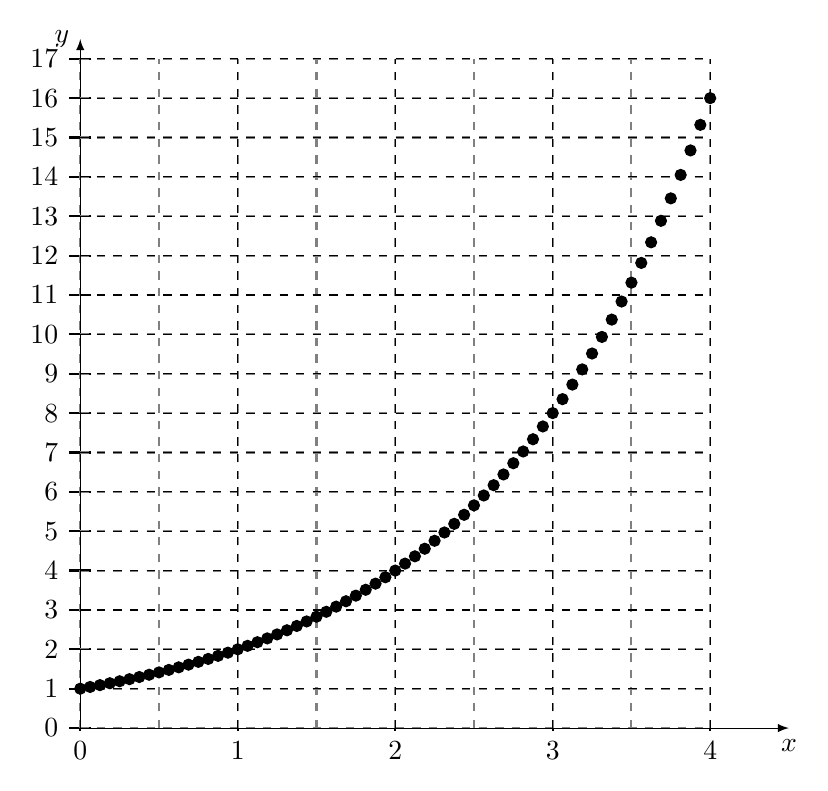
\begin{tikzpicture}[yscale=0.5, xscale=2]
\tkzInit[xmin=0,xmax=4,ymin=0,ymax=17, ystep=1, xstep=1]
\tkzAxeY
\tkzDrawX
\tkzLabelX
   \begin{scope}[dashed]
     \tkzGrid[color=black,sub, subystep=1, subxstep=0.5]
   \end{scope}
\tkzSetUpPoint[size = 4]
\global\edef\tkzFctLast{(exp(x*ln(2)))}
\foreach \va in {0,0.0625,...,4}{%
  \tkzDefPointByFct[draw](\va)
}
\end{tikzpicture}
\end{document}
